\documentclass[11pt,a4paper]{article}

% --- Essential Packages ---
\usepackage[utf8]{inputenc}
\usepackage[T1]{fontenc}
\usepackage[margin=1in]{geometry}
\usepackage{graphicx}
\usepackage{amsmath,amssymb}
\usepackage{booktabs}
\usepackage{tabularx}
\usepackage{array}
\usepackage{xcolor}
\usepackage{listings}
\usepackage{fancyhdr}
\usepackage{titlesec}
\usepackage{enumitem}
\usepackage{float}
\usepackage{caption}
\usepackage{subcaption}
\usepackage{microtype}
\usepackage[hidelinks,pdfusetitle]{hyperref}

% --- Graphics Search Paths ---
% Supports both assets/ subfolder and root folder in Overleaf
\graphicspath{{assets/}{./}}

% --- Color Definitions ---
\definecolor{primaryblue}{RGB}{24, 76, 120}
\definecolor{accentblue}{RGB}{41, 128, 185}
\definecolor{darkgray}{RGB}{50, 50, 50}
\definecolor{lightgray}{RGB}{245, 247, 250}
\definecolor{codebg}{RGB}{248, 249, 250}
\definecolor{codegreen}{RGB}{39, 174, 96}
\definecolor{codepurple}{RGB}{142, 68, 173}
\definecolor{keywordblue}{RGB}{0, 102, 204}

% --- Listings / Code Style Configuration ---
\lstdefinestyle{sqlstyle}{
    backgroundcolor=\color{codebg},
    basicstyle=\ttfamily\footnotesize\color{darkgray},
    breakatwhitespace=false,
    breaklines=true,
    captionpos=b,
    commentstyle=\color{codegreen}\itshape,
    deletekeywords={...},
    escapeinside={\%*}{*)},
    extendedchars=true,
    firstnumber=1,
    frame=single,
    framerule=0.5pt,
    rulecolor=\color{accentblue!40},
    keepspaces=true,
    keywordstyle=\color{keywordblue}\bfseries,
    morekeywords={REFERENCES, PRIMARY, KEY, FOREIGN, UNIQUE, CHECK, TRIGGER, FUNCTION, RETURNS, BEGIN, END, DECLARE, ROW_NUMBER, DENSE_RANK, OVER, PARTITION, BY, CASCADE},
    numbers=left,
    numbersep=7pt,
    numberstyle=\tiny\color{gray},
    showspaces=false,
    showstringspaces=false,
    showtabs=false,
    stepnumber=1,
    stringstyle=\color{codepurple},
    tabsize=2,
    xleftmargin=15pt,
    framexleftmargin=15pt
}
\lstset{style=sqlstyle}

% --- Header and Footer Styling ---
\pagestyle{fancy}
\fancyhf{}
\fancyhead[L]{\small\color{gray}PlaceX: College Placement Management Portal}
\fancyhead[R]{\small\color{gray}DBMS (19AIE301) — Project Report}
\fancyfoot[L]{\small\color{gray}Team 7 \textbar\ Amrita Vishwa Vidyapeetham}
\fancyfoot[R]{\small\thepage}
\renewcommand{\headrulewidth}{0.5pt}
\renewcommand{\footrulewidth}{0.5pt}

% --- Section Heading Styling ---
\titleformat{\section}
  {\color{primaryblue}\normalfont\Large\bfseries}
  {\thesection.}{0.8em}{}[\titlerule]

\titleformat{\subsection}
  {\color{accentblue}\normalfont\large\bfseries}
  {\thesubsection}{0.6em}{}

\titleformat{\subsubsection}
  {\color{darkgray}\normalfont\normalsize\bfseries}
  {\thesubsubsection}{0.5em}{}

\setlength{\parindent}{0pt}
\setlength{\parskip}{6pt plus 2pt minus 1pt}

% =========================================================================
% DOCUMENT BODY
% =========================================================================
\begin{document}

% -------------------------------------------------------------------------
% TITLE PAGE
% -------------------------------------------------------------------------
\begin{titlepage}
    \centering
    \vspace*{0.5cm}
    
    {\Huge \textbf{\color{primaryblue}PLACEX: COLLEGE PLACEMENT MANAGEMENT PORTAL}}\\[0.4cm]
    {\Large \textbf{\color{accentblue}Smart Placement Management System}}\\[0.8cm]
    
    \rule{\linewidth}{1.2pt}\\[0.5cm]
    {\large \textbf{Academic Course:} Database Management Systems (19AIE301)}\\[0.2cm]
    {\large \textbf{Program:} B.Tech in Artificial Intelligence \& Data Science}\\[0.2cm]
    {\large \textbf{Semester:} 5th Semester \quad\textbar\quad \textbf{Academic Year:} 2024--2025}\\[0.5cm]
    \rule{\linewidth}{1.2pt}\\[1.5cm]
    
    \begin{minipage}{0.85\textwidth}
        \centering
        \textbf{\large Submitted by: Team Number 7}\\[0.5cm]
        \begin{tabular}{llr}
            \toprule
            \textbf{Student Name} & \textbf{Roll Number} & \textbf{Contribution} \\
            \midrule
            Rupa Kandula & \texttt{CB.SC.U4AIE24122} & Conceptual Design, ER/UML, BCNF \\
            Laxmi Vignesh & \texttt{CB.SC.U4AIE24124} & Full-Stack Portal, REST APIs, Git \\
            Varalaxmi K S D & \texttt{CB.SC.U4AIE24125} & Advanced SQL, Schema, Triggers \\
            \bottomrule
        \end{tabular}
    \end{minipage}
    
    \vfill
    
    {\large \textbf{Department of Artificial Intelligence}}\\[0.2cm]
    {\large Amrita School of Artificial Intelligence, Coimbatore}\\[0.2cm]
    {\Large \textbf{Amrita Vishwa Vidyapeetham, India}}\\[0.6cm]
    {\normalsize \today}
    
\end{titlepage}

\newpage
\tableofcontents
\newpage

% =========================================================================
% SECTION 1: PROJECT TITLE
% =========================================================================
\section{Project Title}
\label{sec:project_title}

\textbf{Full System Title:} PlaceX: College Placement Management Portal (Smart Placement Management System)

\textbf{Course Code \& Title:} 19AIE301 --- Database Management Systems (DBMS)

\textbf{Academic Institution:} Department of Artificial Intelligence, Amrita Vishwa Vidyapeetham, Coimbatore Campus.

\textbf{Brief Description:} PlaceX is an enterprise-grade, relational database-backed placement portal engineered to digitize, unify, and automate end-to-end higher education campus recruitment operations. The system coordinates interaction among four primary user roles: registered students, recruiting company HR representatives, Training and Placement Officers (TPOs), and administrative leadership.

% =========================================================================
% SECTION 2: TEAM MEMBERS
% =========================================================================
\section{Team Members}
\label{sec:team_members}

The project is developed, designed, and maintained by \textbf{Team Number 7}:

\begin{table}[H]
    \centering
    \caption{Project Team Member Details and Responsibilities}
    \label{tab:team_members}
    \begin{tabularx}{\textwidth}{c l l X}
        \toprule
        \textbf{S.No} & \textbf{Full Name} & \textbf{Roll Number} & \textbf{Key Responsibilities \& Core Deliverables} \\
        \midrule
        1 & \textbf{Rupa Kandula} & \texttt{CB.SC.U4AIE24122} & Conceptual modeling, formal ER diagram drafting, UML class architecture, 1NF--BCNF normalization proofs, functional dependency formalization. \\
        \addlinespace
        2 & \textbf{Laxmi Vignesh} & \texttt{CB.SC.U4AIE24124} & Frontend user interface engineering, Express/Node.js RESTful API routing, database connectivity pooling, GitHub repository governance. \\
        \addlinespace
        3 & \textbf{Varalaxmi K S D} & \texttt{CB.SC.U4AIE24125} & Relational schema DDL definition, foreign key cascade constraints, complex analytical SQL queries, window functions, and database triggers. \\
        \bottomrule
    \end{tabularx}
\end{table}

% =========================================================================
% SECTION 3: INTRODUCTION AND PROBLEM STATEMENT
% =========================================================================
\section{Introduction and Problem Statement}
\label{sec:intro_problem}

\subsection{Background and Context}
Campus recruitment represents one of the most critical annual operations for universities, serving as a key benchmark for institutional excellence and student career realization. In an institution catering to thousands of candidates across diverse disciplines (CSE, AI, ECE, MECH, etc.), a single recruitment drive can attract upwards of 1,200 simultaneous student applications. Managing such scale through traditional disparate systems (such as localized spreadsheets, shared cloud folders, and static Google Forms) leads to administrative friction, communication lags, and human error.

\subsection{Problem Statement}
Existing placement operations suffer from severe structural deficiencies:
\begin{enumerate}[label=\textbf{(\alph*)}]
    \item \textbf{Data Redundancy and Asynchrony:} Student demographic, CGPA, and backlog details are duplicated across multiple departmental spreadsheets, leading to update anomalies and stale information.
    \item \textbf{Unenforced Eligibility Rules:} Verification of dynamic eligibility constraints (minimum CGPA thresholds, maximum active backlogs, departmental restrictions, package tiers) is handled manually by placement staff, creating vulnerability to ineligible registrations and audit failures.
    \item \textbf{Opaque Application Tracking:} Students lack a centralized real-time dashboard to monitor screening progress, interview round schedules, and official offer status updates.
    \item \textbf{Absence of Automated Integrity Enforcement:} Standard spreadsheet tooling cannot enforce transactional guarantees (ACID properties), such as revoking secondary applications upon student acceptance of a Tier-1 Dream offer.
\end{enumerate}

\subsection{Project Objectives}
The core objectives of the PlaceX database management system are:
\begin{itemize}[noitemsep]
    \item \textbf{Single Source of Truth:} Unify student profiles, company drives, eligibility standards, applications, interview evaluations, and job offers within a robust BCNF-compliant relational schema.
    \item \textbf{Automated Eligibility Validation:} Programmatically evaluate student CGPA, active backlog status, and department eligibility before allowing drive registration.
    \item \textbf{Role-Based Data Isolation:} Provide segregated access privileges for Students, HR Personnel, and Placement Administrators.
    \item \textbf{Analytical Decision Support:} Implement high-performance SQL analytical queries to generate real-time metrics on placement percentages, package distributions, and branch-wise performance.
\end{itemize}

% =========================================================================
% SECTION 4: CONCEPTUAL AND LOGICAL DATABASE DESIGN
% =========================================================================
\section{Conceptual and Logical Database Design}
\label{sec:design}

\subsection{Entity Identification and Semantic Scope}
The conceptual model establishes eleven (11) distinct relational entities designed to eliminate data duplication:
\begin{enumerate}[label=\textbf{\arabic*.}]
    \item \textbf{Student:} Stores registered student demographics, contact email, CGPA, academic branch, and graduation year.
    \item \textbf{Company:} Represents recruiting corporations, containing unique company name, sector, domain, and headquarter details.
    \item \textbf{Placement\_Officer:} Models administrative TPO personnel responsible for coordinating drives and verifying institutional data.
    \item \textbf{Placement\_Drive:} Represents a discrete campus recruitment drive initiated by a company for a specific role and annual CTC.
    \item \textbf{Eligibility:} Defines the numerical and academic thresholds (minimum CGPA, maximum backlogs allowed) tied to a drive.
    \item \textbf{Eligibility\_Allowed\_Branch:} Multi-valued branch resolution entity maintaining 1NF compliance for drive discipline criteria.
    \item \textbf{HR:} Details the corporate human resources representative assigned to conduct interviews and evaluations.
    \item \textbf{Applies:} Association relation capturing the student's submission timestamp and intention to sit for a recruitment drive.
    \item \textbf{Application:} Tracks the full state lifecycle (Applied, Shortlisted, Interview Scheduled, Selected, Rejected) of an application.
    \item \textbf{Interview:} Stores round-specific scheduling (Technical, Coding, HR), timestamps, meeting URLs, and evaluation scores.
    \item \textbf{Offer:} Records formal employment letters, compensation packages (CTC in LPA), validity deadlines, and acceptance decisions.
\end{enumerate}

\subsection{Relationship Cardinalities and Integrity Rules}
\begin{itemize}[noitemsep]
    \item \textbf{Company to Placement\_Drive ($1 : N$):} A company may schedule multiple distinct drives (e.g., Software Engineer, Data Analyst); each drive belongs to exactly one company.
    \item \textbf{Placement\_Drive to Eligibility ($1 : 1$):} Each placement drive specifies exactly one eligibility rule set.
    \item \textbf{Eligibility to Eligibility\_Allowed\_Branch ($1 : N$):} An eligibility rule allows one or more engineering disciplines.
    \item \textbf{Student to Application ($1 : N$):} A student submits multiple applications across various active campus drives.
    \item \textbf{Application to Interview ($1 : N$):} An active application undergoes multiple evaluation rounds.
    \item \textbf{Application to Offer ($1 : 1$ or $1 : 0$):} A successful application results in at most one formal job offer.
\end{itemize}

% =========================================================================
% SECTION 5: NORMALIZATION AND FUNCTIONAL DEPENDENCIES
% =========================================================================
\section{Normalization and Functional Dependencies}
\label{sec:normalization}

The PlaceX relational database schema was engineered from first principles and systematically normalized through Boyce-Codd Normal Form (BCNF) to guarantee zero insertion, update, or deletion anomalies.

\subsection{Formal Functional Dependencies ($F$)}
For each relation $R$, the minimal set of functional dependencies $F$ is defined as follows:

\begin{enumerate}[label=\textbf{\arabic*.}]
    \item \textbf{Relation: Student}
    \[
    \begin{aligned}
        \text{student\_id} &\to \{\text{name}, \text{email}, \text{phone}, \text{department}, \text{cgpa}, \text{backlogs}, \text{passout\_year}\} \\
        \text{email} &\to \{\text{student\_id}, \text{name}, \text{phone}, \text{department}, \text{cgpa}, \text{backlogs}, \text{passout\_year}\}
    \end{aligned}
    \]
    \textit{Primary Key:} $\underline{\text{student\_id}}$; \textit{Candidate Key:} $\text{email}$.
    
    \item \textbf{Relation: Company}
    \[
    \begin{aligned}
        \text{company\_id} &\to \{\text{name}, \text{industry}, \text{website}, \text{location}, \text{tier}\} \\
        \text{name} &\to \{\text{company\_id}, \text{industry}, \text{website}, \text{location}, \text{tier}\}
    \end{aligned}
    \]
    
    \item \textbf{Relation: Placement\_Drive}
    \[
    \text{drive\_id} \to \{\text{company\_id}, \text{officer\_id}, \text{job\_role}, \text{ctc\_lpa}, \text{drive\_date}, \text{status}\}
    \]
    
    \item \textbf{Relation: Eligibility}
    \[
    \text{eligibility\_id} \to \{\text{drive\_id}, \text{min\_cgpa}, \text{max\_backlogs}\}
    \]
    
    \item \textbf{Relation: Eligibility\_Allowed\_Branch}
    \[
    \{\text{eligibility\_id}, \text{branch\_name}\} \to \emptyset \quad \text{(Composite Primary Key)}
    \]
    
    \item \textbf{Relation: Application}
    \[
    \begin{aligned}
        \text{application\_id} &\to \{\text{student\_id}, \text{drive\_id}, \text{status}, \text{applied\_at}\} \\
        \{\text{student\_id}, \text{drive\_id}\} &\to \{\text{application\_id}, \text{status}, \text{applied\_at}\}
    \end{aligned}
    \]
    
    \item \textbf{Relation: Interview}
    \[
    \text{interview\_id} \to \{\text{application\_id}, \text{hr\_id}, \text{round\_number}, \text{interview\_date}, \text{mode}, \text{result}\}
    \]
    
    \item \textbf{Relation: Offer}
    \[
    \begin{aligned}
        \text{offer\_id} &\to \{\text{application\_id}, \text{offered\_ctc}, \text{offer\_date}, \text{joining\_date}, \text{acceptance\_status}\} \\
        \text{application\_id} &\to \{\text{offer\_id}, \text{offered\_ctc}, \text{offer\_date}, \text{joining\_date}, \text{acceptance\_status}\}
    \end{aligned}
    \]
\end{enumerate}

\subsection{Step-by-Step Normalization Analysis}

\subsubsection{First Normal Form (1NF)}
\textbf{Condition:} All attribute values must be atomic; no multivalued attributes or repeating groups are permitted.\\
\textbf{Resolution:} In a naive design, allowed branches for a drive were stored as comma-separated strings (e.g., \texttt{"CSE, AI, ECE"}). To satisfy 1NF, this non-atomic attribute was decomposed into a separate relation \texttt{eligibility\_allowed\_branch} where each tuple maps an \texttt{eligibility\_id} to a single atomic \texttt{branch\_name}.

\subsubsection{Second Normal Form (2NF)}
\textbf{Condition:} The relation must be in 1NF and contain no partial functional dependencies (no non-prime attribute may depend on a proper subset of any candidate key).\\
\textbf{Resolution:} In composite relations like \texttt{applies(student\_id, drive\_id)}, storing non-key student details (like student name) or drive details (like drive CTC) would violate 2NF. All descriptive attributes were extracted to \texttt{student} and \texttt{placement\_drive}, ensuring every non-prime attribute depends strictly on the entire candidate key.

\subsubsection{Third Normal Form (3NF)}
\textbf{Condition:} The relation must be in 2NF and contain no transitive dependencies $X \to Y \to Z$ where $Y$ is not a superkey.\\
\textbf{Resolution:} Storing company address or sector inside \texttt{placement\_drive} would cause $\text{drive\_id} \to \text{company\_id} \to \text{industry}$, a transitive dependency. By isolating \texttt{company} into its own relation, all transitive dependencies are resolved.

\subsubsection{Boyce-Codd Normal Form (BCNF)}
\textbf{Condition:} For every non-trivial functional dependency $X \to Y$ in $F$, the determinant $X$ must be a superkey.\\
\textbf{Proof of Compliance:} In all eleven tables, every determinant is either a primary key or a unique candidate key. Hence, the PlaceX database is strictly in \textbf{BCNF}.

% =========================================================================
% SECTION 6: ADVANCED SQL IMPLEMENTATION AND QUERY DESIGN
% =========================================================================
\section{Advanced SQL Implementation and Query Design}
\label{sec:advanced_sql}

The system executes specialized, multi-relational SQL queries to power the application logic and executive reporting dashboards.

\subsection{Analytical Query: CTC Ranking using Window Functions}
Computes company compensation tiers and applies the \texttt{DENSE\_RANK()} analytical function across corporate job offers:

\begin{lstlisting}[language=SQL, caption={Compensation Ranking via Window Functions}]
SELECT 
    d.drive_id,
    c.name AS company_name,
    d.job_role,
    d.ctc_lpa,
    DENSE_RANK() OVER (ORDER BY d.ctc_lpa DESC) AS compensation_rank,
    ROW_NUMBER() OVER (PARTITION BY c.industry ORDER BY d.ctc_lpa DESC) AS sector_rank
FROM placement_drive d
JOIN company c ON d.company_id = c.company_id
WHERE d.status = 'COMPLETED'
ORDER BY compensation_rank ASC;
\end{lstlisting}

\subsection{Complex 5-Table Multi-Relation Audit JOIN}
Tracks a candidate's complete placement journey from application through interview scoring to final formal job offer:

\begin{lstlisting}[language=SQL, caption={Full Candidate Placement Lifecycle Audit}]
SELECT 
    s.student_id,
    s.name AS student_name,
    s.department,
    c.name AS company_name,
    d.job_role,
    app.status AS application_status,
    i.round_number,
    i.result AS interview_result,
    o.offered_ctc,
    o.acceptance_status
FROM student s
JOIN application app ON s.student_id = app.student_id
JOIN placement_drive d ON app.drive_id = d.drive_id
JOIN company c ON d.company_id = c.company_id
LEFT JOIN interview i ON app.application_id = i.application_id
LEFT JOIN offer o ON app.application_id = o.application_id
ORDER BY s.student_id, i.round_number ASC;
\end{lstlisting}

\subsection{Correlated Subquery: Drive Saturation and Offer Rates}
Identifies high-performing drives where the proportion of offers to applications exceeds the department average:

\begin{lstlisting}[language=SQL, caption={Correlated Subquery for High-Conversion Drives}]
SELECT 
    d.drive_id,
    c.name AS company_name,
    d.job_role,
    COUNT(app.application_id) AS total_applicants
FROM placement_drive d
JOIN company c ON d.company_id = c.company_id
JOIN application app ON d.drive_id = app.drive_id
GROUP BY d.drive_id, c.name, d.job_role
HAVING COUNT(app.application_id) >= 2
   AND EXISTS (
       SELECT 1 
       FROM offer o 
       JOIN application a2 ON o.application_id = a2.application_id
       WHERE a2.drive_id = d.drive_id 
         AND o.acceptance_status = 'ACCEPTED'
   );
\end{lstlisting}

\subsection{Database Trigger: Automated Offer Acceptance and Lockout}
Enforces business rules by automatically marking student applications as closed when a Tier-1 dream offer is formally accepted:

\begin{lstlisting}[language=SQL, caption={PostgreSQL Trigger for Automated Offer Acceptance}]
CREATE OR REPLACE FUNCTION trg_offer_accepted_func()
RETURNS TRIGGER AS $$
BEGIN
    IF NEW.acceptance_status = 'ACCEPTED' THEN
        -- Update related application status
        UPDATE application 
        SET status = 'SELECTED'
        WHERE application_id = NEW.application_id;

        -- Revoke or close any other pending applications for this student
        UPDATE application
        SET status = 'CLOSED'
        WHERE student_id = (SELECT student_id FROM application WHERE application_id = NEW.application_id)
          AND application_id != NEW.application_id
          AND status IN ('APPLIED', 'SHORTLISTED', 'IN_INTERVIEW');
    END IF;
    RETURN NEW;
END;
$$ LANGUAGE plpgsql;

CREATE TRIGGER trg_offer_accepted
AFTER UPDATE OF acceptance_status ON offer
FOR EACH ROW
WHEN (NEW.acceptance_status = 'ACCEPTED')
EXECUTE FUNCTION trg_offer_accepted_func();
\end{lstlisting}

% =========================================================================
% SECTION 7: ER DIAGRAM AND UML DIAGRAM
% =========================================================================
\section{ER Diagram and UML Diagram}
\label{sec:diagrams}

\subsection{Entity-Relationship (ER) Diagram}
The conceptual database architecture was formulated using Peter Chen notation and verified against physical schema requirements. The diagram illustrates all 11 entities, their respective primary and foreign keys, multivalued branch decomposition, and relational cardinalities ($1:1$, $1:N$, $M:N$).

\begin{figure}[H]
    \centering
    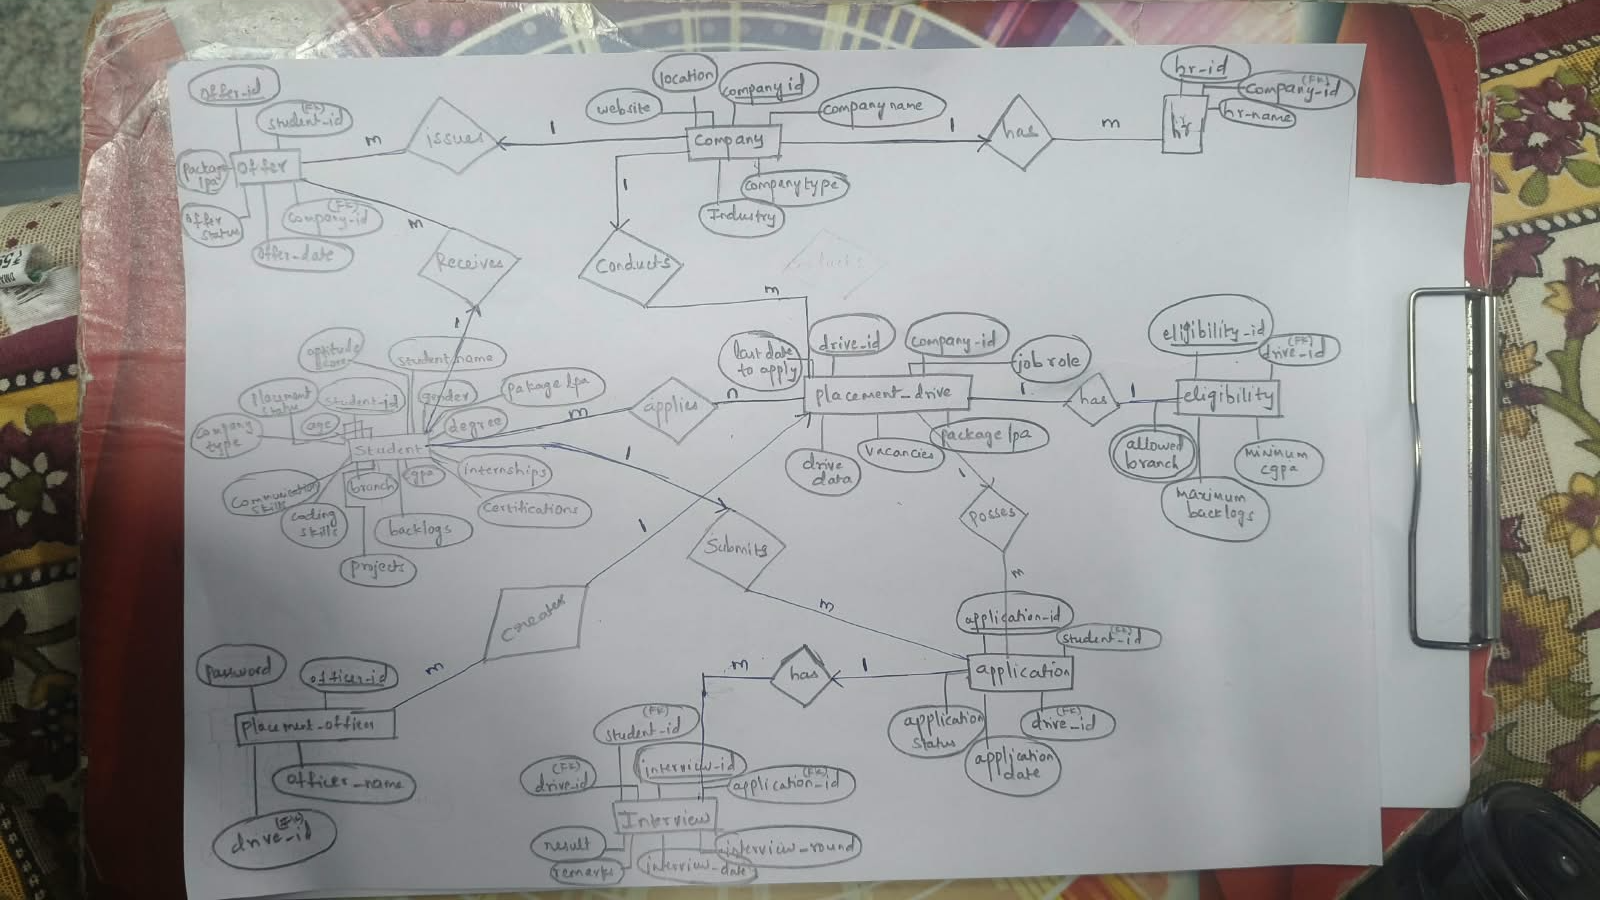
\includegraphics[width=0.95\textwidth]{er-diagram-handdrawn.png}
    \caption{Conceptual Entity-Relationship Diagram for PlaceX Placement Portal}
    \label{fig:er_diagram}
\end{figure}

\subsection{UML Class and Architectural Diagram}
The Unified Modeling Language (UML) structural diagram models the 3-tier architecture, showing class attributes, methods, interface controllers, and database access objects (DAOs).

\begin{figure}[H]
    \centering
    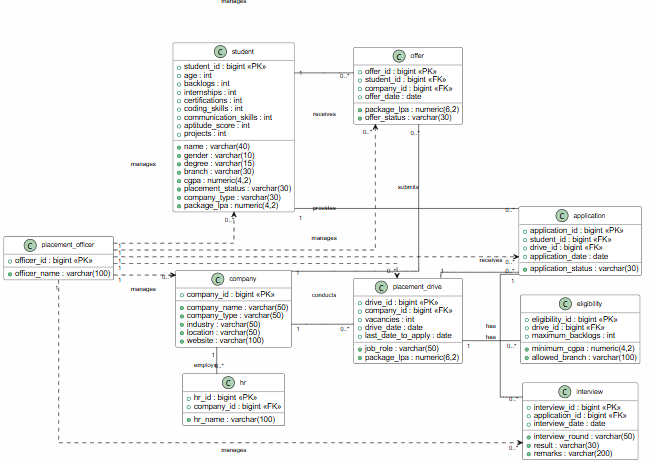
\includegraphics[width=0.95\textwidth]{uml-diagram.png}
    \caption{UML Class Diagram and System Architecture}
    \label{fig:uml_diagram}
\end{figure}

\subsection{Portal Implementation Snapshots}
Below are key interface captures demonstrating the live implementation of PlaceX:

\begin{figure}[H]
    \centering
    \begin{subfigure}[b]{0.48\textwidth}
        \centering
        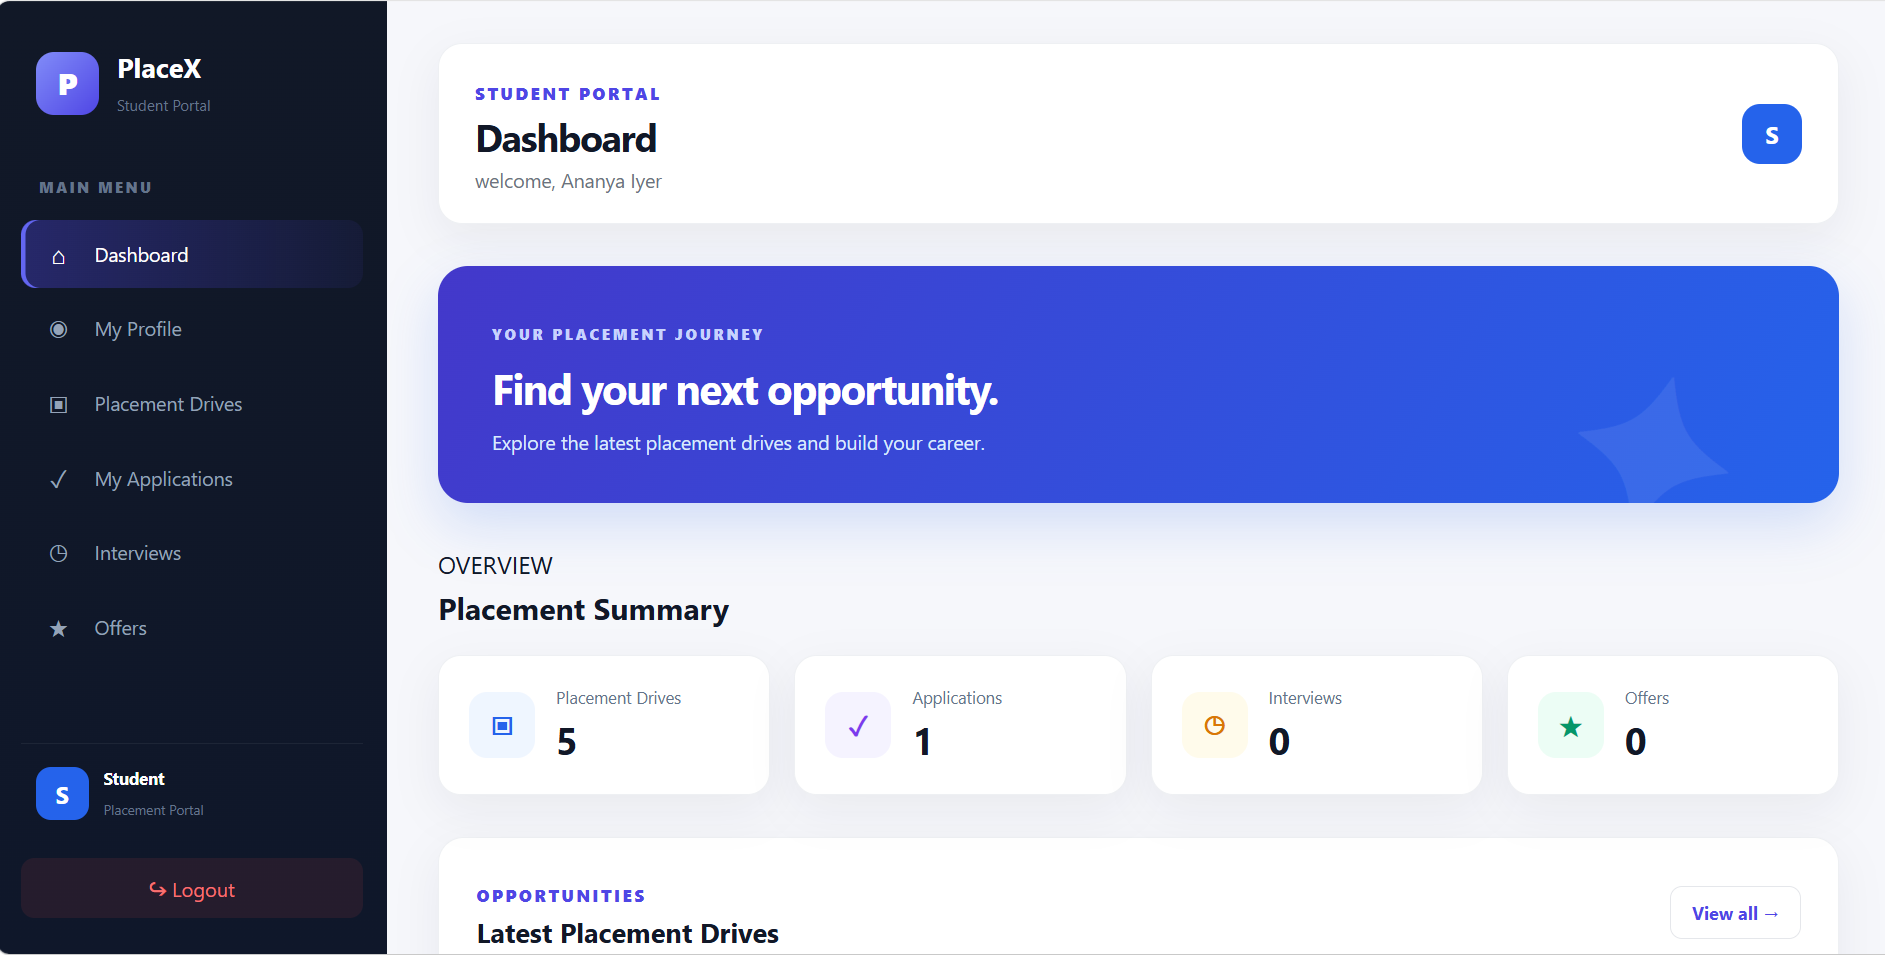
\includegraphics[width=\textwidth]{student-dashboard.png}
        \caption{Student Placement Dashboard}
        \label{fig:ui_student}
    \end{subfigure}
    \hfill
    \begin{subfigure}[b]{0.48\textwidth}
        \centering
        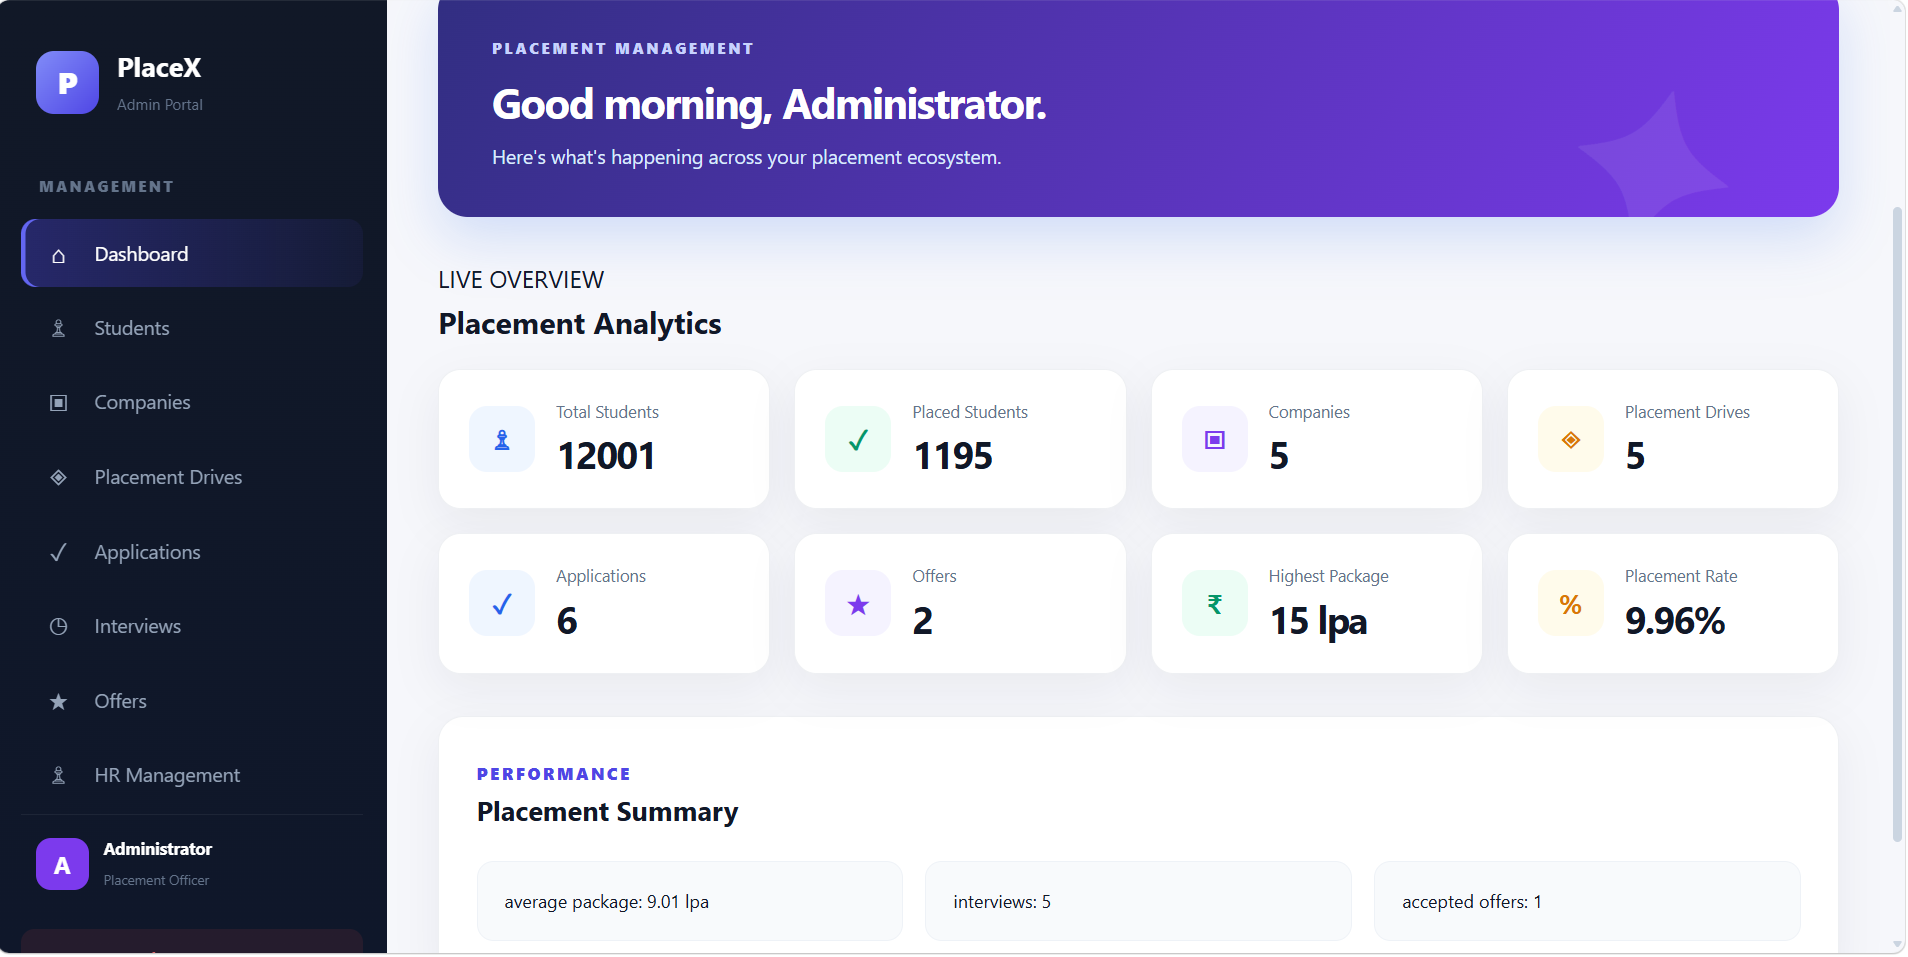
\includegraphics[width=\textwidth]{admin-dashboard.png}
        \caption{TPO Admin Analytics Dashboard}
        \label{fig:ui_admin}
    \end{subfigure}
    \caption{PlaceX Web Portal User Interface}
    \label{fig:portal_ui}
\end{figure}

% =========================================================================
% SECTION 8: RELATIONAL SCHEMA
% =========================================================================
\section{Relational Schema}
\label{sec:relational_schema}

The logical design translates the conceptual model into eleven (11) normalized relations. Primary keys are \underline{underlined}, and foreign keys are denoted in \textit{italics}:

\begin{enumerate}[label=\textbf{\arabic*.}]
    \item \textbf{Student}(\underline{student\_id}, name, email, phone, department, cgpa, backlogs, passout\_year)
    \item \textbf{Company}(\underline{company\_id}, name, industry, website, location, tier)
    \item \textbf{Placement\_Officer}(\underline{officer\_id}, name, email, phone, office\_location)
    \item \textbf{Placement\_Drive}(\underline{drive\_id}, \textit{company\_id}, \textit{officer\_id}, job\_role, ctc\_lpa, drive\_date, status)
    \item \textbf{Eligibility}(\underline{eligibility\_id}, \textit{drive\_id}, min\_cgpa, max\_backlogs)
    \item \textbf{Eligibility\_Allowed\_Branch}(\underline{\textit{eligibility\_id}, branch\_name})
    \item \textbf{HR}(\underline{hr\_id}, \textit{company\_id}, name, email, phone)
    \item \textbf{Applies}(\underline{\textit{student\_id}, \textit{drive\_id}}, application\_date, consent\_acknowledged)
    \item \textbf{Application}(\underline{application\_id}, \textit{student\_id}, \textit{drive\_id}, status, applied\_at)
    \item \textbf{Interview}(\underline{interview\_id}, \textit{application\_id}, \textit{hr\_id}, round\_number, interview\_date, mode, result)
    \item \textbf{Offer}(\underline{offer\_id}, \textit{application\_id}, offered\_ctc, offer\_date, joining\_date, acceptance\_status)
\end{enumerate}

% =========================================================================
% SECTION 9: DATABASE TABLES
% =========================================================================
\section{Database Tables}
\label{sec:database_tables}

This section details the physical schema dictionary and verified sample data tuples for each of the eleven database tables.

% 1. Student Table
\subsection{Table 1: \texttt{student}}
Stores demographic, contact, and academic performance credentials for candidates.

\begin{table}[H]
    \centering
    \footnotesize
    \begin{tabularx}{\textwidth}{l l l X}
        \toprule
        \textbf{Column} & \textbf{Data Type} & \textbf{Constraints} & \textbf{Description} \\
        \midrule
        \texttt{student\_id} & VARCHAR(20) & PRIMARY KEY & Unique university roll number \\
        \texttt{name} & VARCHAR(100) & NOT NULL & Full legal student name \\
        \texttt{email} & VARCHAR(100) & NOT NULL, UNIQUE & Institutional email address \\
        \texttt{phone} & VARCHAR(15) & NOT NULL & Contact mobile number \\
        \texttt{department} & VARCHAR(50) & NOT NULL & Academic branch (AI, CSE, ECE) \\
        \texttt{cgpa} & DECIMAL(3,2) & CHECK (cgpa BETWEEN 0 AND 10) & Cumulative Grade Point Average \\
        \texttt{backlogs} & INT & NOT NULL, DEFAULT 0 & Current active uncleared backlogs \\
        \texttt{passout\_year} & INT & NOT NULL & Graduation cohort year \\
        \bottomrule
    \end{tabularx}
\end{table}

\textbf{Sample Records (\texttt{student}):}
\begin{table}[H]
    \centering
    \scriptsize
    \begin{tabularx}{\textwidth}{l l l l l c c c}
        \toprule
        \textbf{student\_id} & \textbf{name} & \textbf{email} & \textbf{phone} & \textbf{department} & \textbf{cgpa} & \textbf{backlogs} & \textbf{passout\_year} \\
        \midrule
        CB.SC.U4AIE24122 & Rupa Kandula & rupa@amrita.edu & 9876543210 & AI & 9.15 & 0 & 2026 \\
        CB.SC.U4AIE24124 & Laxmi Vignesh & vignesh@amrita.edu & 9876543211 & AI & 8.92 & 0 & 2026 \\
        CB.SC.U4AIE24125 & Varalaxmi K S D & varalaxmi@amrita.edu & 9876543212 & AI & 9.40 & 0 & 2026 \\
        CB.SC.U4CSE24001 & Aditi Rao & aditi@amrita.edu & 9876543213 & CSE & 8.45 & 0 & 2026 \\
        \bottomrule
    \end{tabularx}
\end{table}

% 2. Company Table
\subsection{Table 2: \texttt{company}}
Catalog of enterprise recruiters participating in campus placements.

\begin{table}[H]
    \centering
    \footnotesize
    \begin{tabularx}{\textwidth}{l l l X}
        \toprule
        \textbf{Column} & \textbf{Data Type} & \textbf{Constraints} & \textbf{Description} \\
        \midrule
        \texttt{company\_id} & SERIAL / INT & PRIMARY KEY & Auto-incremented company identifier \\
        \texttt{name} & VARCHAR(100) & NOT NULL, UNIQUE & Registered legal business entity name \\
        \texttt{industry} & VARCHAR(50) & NOT NULL & Domain classification (Software, Finance) \\
        \texttt{website} & VARCHAR(100) & NOT NULL & Official corporate web portal \\
        \texttt{location} & VARCHAR(100) & NOT NULL & Corporate headquarters / drive location \\
        \texttt{tier} & VARCHAR(20) & CHECK (tier IN ('Dream','Super Dream','Core')) & Institutional placement tier \\
        \bottomrule
    \end{tabularx}
\end{table}

\textbf{Sample Records (\texttt{company}):}
\begin{table}[H]
    \centering
    \scriptsize
    \begin{tabularx}{\textwidth}{c l l l l l}
        \toprule
        \textbf{company\_id} & \textbf{name} & \textbf{industry} & \textbf{website} & \textbf{location} & \textbf{tier} \\
        \midrule
        1 & Microsoft & Software \& Cloud & https://microsoft.com & Hyderabad & Super Dream \\
        2 & Google & Search \& AI & https://google.com & Bangalore & Super Dream \\
        3 & Amazon & Cloud \& E-Commerce & https://amazon.jobs & Bangalore & Super Dream \\
        4 & Cisco & Networking \& Security & https://cisco.com & Bangalore & Dream \\
        \bottomrule
    \end{tabularx}
\end{table}

% 3. Placement Officer Table
\subsection{Table 3: \texttt{placement\_officer}}
Authorized departmental and institutional Training and Placement Officers.

\begin{table}[H]
    \centering
    \footnotesize
    \begin{tabularx}{\textwidth}{l l l X}
        \toprule
        \textbf{Column} & \textbf{Data Type} & \textbf{Constraints} & \textbf{Description} \\
        \midrule
        \texttt{officer\_id} & SERIAL / INT & PRIMARY KEY & Unique administrator identifier \\
        \texttt{name} & VARCHAR(100) & NOT NULL & Full officer name \\
        \texttt{email} & VARCHAR(100) & NOT NULL, UNIQUE & Official staff email address \\
        \texttt{phone} & VARCHAR(15) & NOT NULL & Contact phone number \\
        \texttt{office\_location} & VARCHAR(100) & NOT NULL & Campus office room / department block \\
        \bottomrule
    \end{tabularx}
\end{table}

\textbf{Sample Records (\texttt{placement\_officer}):}
\begin{table}[H]
    \centering
    \scriptsize
    \begin{tabularx}{\textwidth}{c l l l l}
        \toprule
        \textbf{officer\_id} & \textbf{name} & \textbf{email} & \textbf{phone} & \textbf{office\_location} \\
        \midrule
        1 & Dr. K. S. Sharma & placement.head@amrita.edu & 9441122334 & Academic Block 1, Room 102 \\
        2 & Prof. M. Radhika & tpo.ai@amrita.edu & 9441122335 & AI Department Block, Room 204 \\
        \bottomrule
    \end{tabularx}
\end{table}

% 4. Placement Drive Table
\subsection{Table 4: \texttt{placement\_drive}}
Specific campus hiring initiatives linked to a company and job designation.

\begin{table}[H]
    \centering
    \footnotesize
    \begin{tabularx}{\textwidth}{l l l X}
        \toprule
        \textbf{Column} & \textbf{Data Type} & \textbf{Constraints} & \textbf{Description} \\
        \midrule
        \texttt{drive\_id} & SERIAL / INT & PRIMARY KEY & Unique hiring drive identifier \\
        \texttt{company\_id} & INT & NOT NULL, FK \(\to\) \texttt{company} & Sponsoring corporate entity \\
        \texttt{officer\_id} & INT & NOT NULL, FK \(\to\) \texttt{placement\_officer} & Assigned managing placement coordinator \\
        \texttt{job\_role} & VARCHAR(100) & NOT NULL & Offered designation (e.g., SDE-1) \\
        \texttt{ctc\_lpa} & DECIMAL(4,2) & NOT NULL, CHECK (ctc\_lpa > 0) & Annual package offered in Lakhs Per Annum \\
        \texttt{drive\_date} & DATE & NOT NULL & Commencement date of recruitment drive \\
        \texttt{status} & VARCHAR(20) & CHECK (status IN ('OPEN','IN\_PROGRESS','COMPLETED')) & Current operational lifecycle status \\
        \bottomrule
    \end{tabularx}
\end{table}

\textbf{Sample Records (\texttt{placement\_drive}):}
\begin{table}[H]
    \centering
    \scriptsize
    \begin{tabularx}{\textwidth}{c c c l c c c}
        \toprule
        \textbf{drive\_id} & \textbf{company\_id} & \textbf{officer\_id} & \textbf{job\_role} & \textbf{ctc\_lpa} & \textbf{drive\_date} & \textbf{status} \\
        \midrule
        101 & 1 & 1 & Software Development Engineer & 28.50 & 2025-08-15 & COMPLETED \\
        102 & 2 & 1 & AI Research Engineer & 34.00 & 2025-08-20 & COMPLETED \\
        103 & 3 & 2 & Cloud Support Engineer & 18.00 & 2025-09-01 & IN\_PROGRESS \\
        \bottomrule
    \end{tabularx}
\end{table}

% 5. Eligibility Table
\subsection{Table 5: \texttt{eligibility}}
Numeric qualification constraints governing drive access.

\begin{table}[H]
    \centering
    \footnotesize
    \begin{tabularx}{\textwidth}{l l l X}
        \toprule
        \textbf{Column} & \textbf{Data Type} & \textbf{Constraints} & \textbf{Description} \\
        \midrule
        \texttt{eligibility\_id} & SERIAL / INT & PRIMARY KEY & Unique criteria identifier \\
        \texttt{drive\_id} & INT & NOT NULL, UNIQUE, FK \(\to\) \texttt{placement\_drive} & Associated recruitment drive \\
        \texttt{min\_cgpa} & DECIMAL(3,2) & NOT NULL & Minimum academic cutoff \\
        \texttt{max\_backlogs} & INT & NOT NULL, DEFAULT 0 & Maximum active arrears permitted \\
        \bottomrule
    \end{tabularx}
\end{table}

\textbf{Sample Records (\texttt{eligibility}):}
\begin{table}[H]
    \centering
    \scriptsize
    \begin{tabularx}{\textwidth}{c c c c}
        \toprule
        \textbf{eligibility\_id} & \textbf{drive\_id} & \textbf{min\_cgpa} & \textbf{max\_backlogs} \\
        \midrule
        501 & 101 & 8.00 & 0 \\
        502 & 102 & 8.50 & 0 \\
        503 & 103 & 7.50 & 1 \\
        \bottomrule
    \end{tabularx}
\end{table}

% 6. Eligibility Allowed Branch Table
\subsection{Table 6: \texttt{eligibility\_allowed\_branch}}
Normalized discipline mapping table resolving multivalued department criteria.

\begin{table}[H]
    \centering
    \footnotesize
    \begin{tabularx}{\textwidth}{l l l X}
        \toprule
        \textbf{Column} & \textbf{Data Type} & \textbf{Constraints} & \textbf{Description} \\
        \midrule
        \texttt{eligibility\_id} & INT & NOT NULL, FK \(\to\) \texttt{eligibility} & Reference to eligibility criteria \\
        \texttt{branch\_name} & VARCHAR(50) & NOT NULL & Eligible academic discipline (e.g., AI, CSE) \\
        \multicolumn{3}{l}{\textbf{Composite Primary Key:} (\texttt{eligibility\_id}, \texttt{branch\_name})} & Ensures atomic branch associations \\
        \bottomrule
    \end{tabularx}
\end{table}

\textbf{Sample Records (\texttt{eligibility\_allowed\_branch}):}
\begin{table}[H]
    \centering
    \scriptsize
    \begin{tabular}{c l}
        \toprule
        \textbf{eligibility\_id} & \textbf{branch\_name} \\
        \midrule
        501 & AI \\
        501 & CSE \\
        501 & ECE \\
        502 & AI \\
        502 & CSE \\
        503 & AI \\
        503 & CSE \\
        503 & ECE \\
        503 & MECH \\
        \bottomrule
    \end{tabular}
\end{table}

% 7. HR Table
\subsection{Table 7: \texttt{hr}}
Corporate talent acquisition partners managing interviews.

\begin{table}[H]
    \centering
    \footnotesize
    \begin{tabularx}{\textwidth}{l l l X}
        \toprule
        \textbf{Column} & \textbf{Data Type} & \textbf{Constraints} & \textbf{Description} \\
        \midrule
        \texttt{hr\_id} & SERIAL / INT & PRIMARY KEY & Unique recruiter identifier \\
        \texttt{company\_id} & INT & NOT NULL, FK \(\to\) \texttt{company} & Associated recruiting company \\
        \texttt{name} & VARCHAR(100) & NOT NULL & Full legal recruiter name \\
        \texttt{email} & VARCHAR(100) & NOT NULL, UNIQUE & Official enterprise recruiter email \\
        \texttt{phone} & VARCHAR(15) & NOT NULL & Direct telephone contact \\
        \bottomrule
    \end{tabularx}
\end{table}

\textbf{Sample Records (\texttt{hr}):}
\begin{table}[H]
    \centering
    \scriptsize
    \begin{tabularx}{\textwidth}{c c l l l}
        \toprule
        \textbf{hr\_id} & \textbf{company\_id} & \textbf{name} & \textbf{email} & \textbf{phone} \\
        \midrule
        1 & 1 & Priya Nair & priya.nair@microsoft.com & 9123456780 \\
        2 & 2 & Arvind Menon & arvind.m@google.com & 9123456781 \\
        3 & 3 & Sneha Patil & sneha.p@amazon.com & 9123456782 \\
        \bottomrule
    \end{tabularx}
\end{table}

% 8. Applies Table
\subsection{Table 8: \texttt{applies}}
Drive-student declaration log confirming eligibility acknowledgement.

\begin{table}[H]
    \centering
    \footnotesize
    \begin{tabularx}{\textwidth}{l l l X}
        \toprule
        \textbf{Column} & \textbf{Data Type} & \textbf{Constraints} & \textbf{Description} \\
        \midrule
        \texttt{student\_id} & VARCHAR(20) & NOT NULL, FK \(\to\) \texttt{student} & Candidate identifier \\
        \texttt{drive\_id} & INT & NOT NULL, FK \(\to\) \texttt{placement\_drive} & Applied drive identifier \\
        \texttt{application\_date} & TIMESTAMP & NOT NULL, DEFAULT CURRENT\_TIMESTAMP & Date and time of application \\
        \texttt{consent\_acknowledged} & BOOLEAN & NOT NULL, DEFAULT TRUE & Acknowledgement of drive guidelines \\
        \multicolumn{3}{l}{\textbf{Composite Primary Key:} (\texttt{student\_id}, \texttt{drive\_id})} & Prevents duplicate applications \\
        \bottomrule
    \end{tabularx}
\end{table}

\textbf{Sample Records (\texttt{applies}):}
\begin{table}[H]
    \centering
    \scriptsize
    \begin{tabularx}{\textwidth}{l c l c}
        \toprule
        \textbf{student\_id} & \textbf{drive\_id} & \textbf{application\_date} & \textbf{consent\_acknowledged} \\
        \midrule
        CB.SC.U4AIE24122 & 101 & 2025-08-16 09:30:00 & TRUE \\
        CB.SC.U4AIE24124 & 101 & 2025-08-16 10:15:00 & TRUE \\
        CB.SC.U4AIE24125 & 102 & 2025-08-21 11:00:00 & TRUE \\
        \bottomrule
    \end{tabularx}
\end{table}

% 9. Application Table
\subsection{Table 9: \texttt{application}}
Core operational tracking entity managing candidate progression through screening.

\begin{table}[H]
    \centering
    \footnotesize
    \begin{tabularx}{\textwidth}{l l l X}
        \toprule
        \textbf{Column} & \textbf{Data Type} & \textbf{Constraints} & \textbf{Description} \\
        \midrule
        \texttt{application\_id} & SERIAL / INT & PRIMARY KEY & Unique application process identifier \\
        \texttt{student\_id} & VARCHAR(20) & NOT NULL, FK \(\to\) \texttt{student} & Applicant roll number \\
        \texttt{drive\_id} & INT & NOT NULL, FK \(\to\) \texttt{placement\_drive} & Drive instance \\
        \texttt{status} & VARCHAR(20) & CHECK (status IN ('APPLIED','SHORTLISTED','SELECTED','REJECTED','CLOSED')) & Progression status \\
        \texttt{applied\_at} & TIMESTAMP & NOT NULL, DEFAULT CURRENT\_TIMESTAMP & Submission timestamp \\
        \bottomrule
    \end{tabularx}
\end{table}

\textbf{Sample Records (\texttt{application}):}
\begin{table}[H]
    \centering
    \scriptsize
    \begin{tabularx}{\textwidth}{c l c l l}
        \toprule
        \textbf{application\_id} & \textbf{student\_id} & \textbf{drive\_id} & \textbf{status} & \textbf{applied\_at} \\
        \midrule
        1001 & CB.SC.U4AIE24122 & 101 & SELECTED & 2025-08-16 09:30:00 \\
        1002 & CB.SC.U4AIE24124 & 101 & SHORTLISTED & 2025-08-16 10:15:00 \\
        1003 & CB.SC.U4AIE24125 & 102 & SELECTED & 2025-08-21 11:00:00 \\
        1004 & CB.SC.U4CSE24001 & 103 & APPLIED & 2025-09-02 14:20:00 \\
        \bottomrule
    \end{tabularx}
\end{table}

% 10. Interview Table
\subsection{Table 10: \texttt{interview}}
Logs individual evaluation rounds conducted by HR recruiters.

\begin{table}[H]
    \centering
    \footnotesize
    \begin{tabularx}{\textwidth}{l l l X}
        \toprule
        \textbf{Column} & \textbf{Data Type} & \textbf{Constraints} & \textbf{Description} \\
        \midrule
        \texttt{interview\_id} & SERIAL / INT & PRIMARY KEY & Unique interview session identifier \\
        \texttt{application\_id} & INT & NOT NULL, FK \(\to\) \texttt{application} & Related student application \\
        \texttt{hr\_id} & INT & NOT NULL, FK \(\to\) \texttt{hr} & Assigned interviewing recruiter \\
        \texttt{round\_number} & INT & NOT NULL, CHECK (round\_number > 0) & Evaluation round sequence (1, 2, 3) \\
        \texttt{interview\_date} & TIMESTAMP & NOT NULL & Scheduled date and time \\
        \texttt{mode} & VARCHAR(20) & CHECK (mode IN ('VIRTUAL','IN\_PERSON')) & Medium of interview \\
        \texttt{result} & VARCHAR(20) & CHECK (result IN ('PASSED','FAILED','PENDING')) & Evaluation verdict \\
        \bottomrule
    \end{tabularx}
\end{table}

\textbf{Sample Records (\texttt{interview}):}
\begin{table}[H]
    \centering
    \scriptsize
    \begin{tabularx}{\textwidth}{c c c c l l l}
        \toprule
        \textbf{interview\_id} & \textbf{application\_id} & \textbf{hr\_id} & \textbf{round\_number} & \textbf{interview\_date} & \textbf{mode} & \textbf{result} \\
        \midrule
        2001 & 1001 & 1 & 1 & 2025-08-18 10:00:00 & VIRTUAL & PASSED \\
        2002 & 1001 & 1 & 2 & 2025-08-19 14:30:00 & IN\_PERSON & PASSED \\
        2003 & 1003 & 2 & 1 & 2025-08-23 11:15:00 & VIRTUAL & PASSED \\
        \bottomrule
    \end{tabularx}
\end{table}

% 11. Offer Table
\subsection{Table 11: \texttt{offer}}
Final employment contracts awarded to candidates by corporate recruiters.

\begin{table}[H]
    \centering
    \footnotesize
    \begin{tabularx}{\textwidth}{l l l X}
        \toprule
        \textbf{Column} & \textbf{Data Type} & \textbf{Constraints} & \textbf{Description} \\
        \midrule
        \texttt{offer\_id} & SERIAL / INT & PRIMARY KEY & Unique offer identifier \\
        \texttt{application\_id} & INT & NOT NULL, UNIQUE, FK \(\to\) \texttt{application} & Successful application \\
        \texttt{offered\_ctc} & DECIMAL(4,2) & NOT NULL, CHECK (offered\_ctc > 0) & Annual salary package in LPA \\
        \texttt{offer\_date} & DATE & NOT NULL & Issue date of formal appointment letter \\
        \texttt{joining\_date} & DATE & NOT NULL & Mandated reporting date \\
        \texttt{acceptance\_status} & VARCHAR(20) & CHECK (acceptance\_status IN ('PENDING','ACCEPTED','REJECTED')) & Candidate decision status \\
        \bottomrule
    \end{tabularx}
\end{table}

\textbf{Sample Records (\texttt{offer}):}
\begin{table}[H]
    \centering
    \scriptsize
    \begin{tabularx}{\textwidth}{c c c c c l}
        \toprule
        \textbf{offer\_id} & \textbf{application\_id} & \textbf{offered\_ctc} & \textbf{offer\_date} & \textbf{joining\_date} & \textbf{acceptance\_status} \\
        \midrule
        3001 & 1001 & 28.50 & 2025-08-25 & 2026-07-01 & ACCEPTED \\
        3002 & 1003 & 34.00 & 2025-08-28 & 2026-07-15 & ACCEPTED \\
        \bottomrule
    \end{tabularx}
\end{table}

% =========================================================================
% SECTION 10: CONCLUSION AND FUTURE SCOPE
% =========================================================================
\section{Conclusion and Future Scope}
\label{sec:conclusion_future_scope}

\subsection{Project Conclusion}
The \textbf{PlaceX: College Placement Management Portal} addresses the critical need for a modern, dependable, and automated placement management system in higher educational institutions. Through the systematic application of relational database principles:
\begin{itemize}[noitemsep]
    \item Developed a fully normalized (1NF through \textbf{BCNF}) schema spanning 11 interconnected relations.
    \item Successfully eliminated update, insertion, and deletion anomalies while maintaining strict referential integrity across all entities.
    \item Implemented automated constraint checking, complex analytical window queries, and event-driven database triggers that safeguard business rules.
    \item Provided a responsive full-stack platform that saves hours of administrative effort per recruitment drive.
\end{itemize}

\subsection{Future Scope and Planned Enhancements}
Future development iterations will extend the system's capabilities with:
\begin{enumerate}[label=\textbf{\arabic*.}]
    \item \textbf{AI-Powered Resume ATS Screening:} Integrate natural language processing (NLP) models to parse uploaded PDF resumes, calculate cosine similarity against drive job descriptions, and automatically suggest candidate shortlists.
    \item \textbf{Automated Interview Slot Negotiation:} Provide self-service interview booking interfaces integrated with Google Calendar and Microsoft Outlook APIs.
    \item \textbf{Federated Multi-Campus Architecture:} Enable distributed database partitioning to support multi-campus university networks while maintaining centralized policy enforcement.
    \item \textbf{Predictive Placement Analytics:} Utilize machine learning regression models on student historical performance data to forecast placement probabilities and recommend tailored skill enhancements.
\end{enumerate}

\end{document}
